\documentclass{standalone}
\usepackage{graphicx}
\usepackage{amssymb}
\usepackage{epstopdf}

\usepackage{tikz}
\usetikzlibrary{decorations.markings,arrows.meta}

\begin{document}

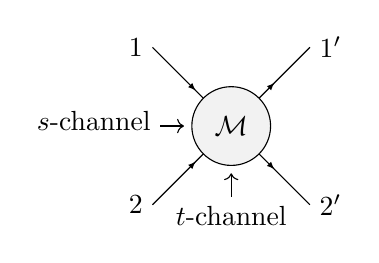
\begin{tikzpicture}[
        decoration={
                markings,
                mark=at position 0.55 with {\arrow[scale=0.7]{latex}}
            }
    ]
    % Line 1
    \draw[postaction={decorate}] (-1,1) node[left] {$1$} -- (0,0);
    \draw[postaction={decorate}] (0,0) -- (1,-1) node[right] {$2'$};

    % Line 2
    \draw[postaction={decorate}] (-1,-1) node[left] {$2$} -- (0,0);
    \draw[postaction={decorate}] (0,0) -- (1,1) node[right] {$1'$};

    % Circle
    \draw[black, fill=gray!10] (0,0) circle (0.5) node[] {$\mathcal{M}$};

    \draw[->, thin] (-0.9,0) -- (-0.6,0);
    \node[anchor=east, yshift=1.7] at (-0.9,0) {$s$-channel};

    \draw[->, thin] (0,-0.9) -- (0,-0.6);
    \node[anchor=north] at (0,-0.9) {$t$-channel};
\end{tikzpicture}

\end{document}
